\documentclass{beamer}
\usepackage{tikz}
\usetikzlibrary{arrows.meta, calc}

% ------------------------------------------------------------------
% This figure has four functionally distinct blocks and three
% semantically distinct buses, so (unlike the byte-level LDR/STR
% diagrams) it keeps the SVG's own colour coding rather than the
% blk/accent two-colour scheme — that coding IS the information here.
% The conventions carried over from the house style: \tikzset named
% styles, sans-serif \lbl labels, thick strokes, {Stealth} arrows, and
% \resizebox to fit the slide.
% ------------------------------------------------------------------
\definecolor{regfill}{HTML}{FFF1B6}
\definecolor{regline}{HTML}{AB9042}
\definecolor{shiftfill}{HTML}{C3E9FF}
\definecolor{shiftline}{HTML}{3F7691}
\definecolor{alufill}{HTML}{D8FFD2}
\definecolor{aluline}{HTML}{4F7D49}
\definecolor{psrfill}{HTML}{ECDCE8}
\definecolor{psrline}{HTML}{CFABCF}
\definecolor{busflag}{HTML}{A84A4A}

\tikzset{
  lbl/.style={text=black},
  flow/.style={-{Stealth[length=2mm]}, thick},
}

\begin{document}

\begin{frame}{ARM Datapath: The Barrel Shifter}
\centering
\resizebox{0.88\textwidth}{!}{%
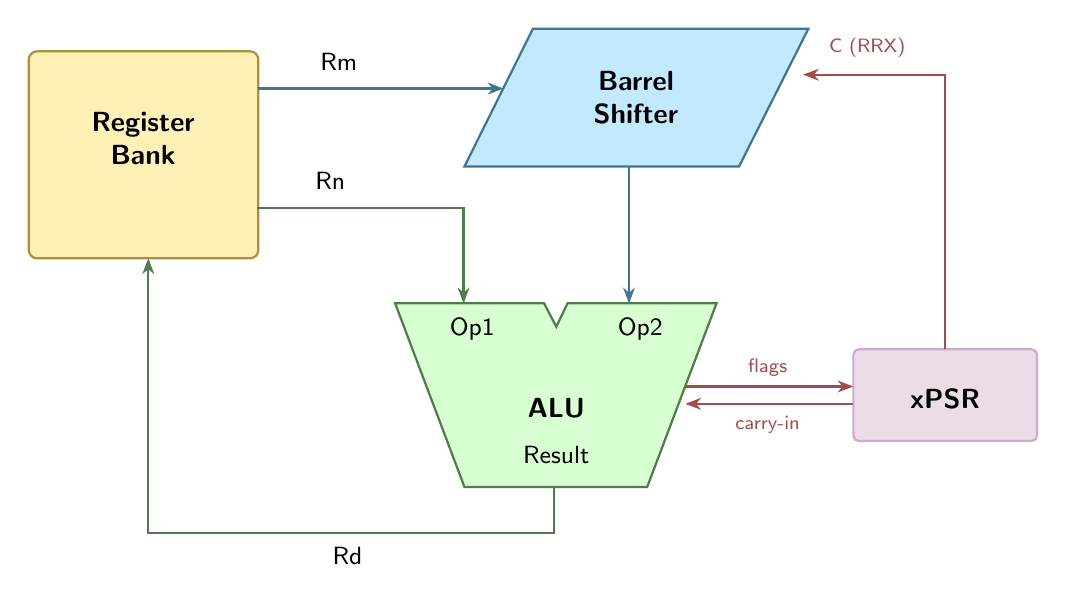
\begin{tikzpicture}[xscale=0.11,yscale=-0.11]

% --- Register Bank ---
\draw[thick, draw=regline, fill=regfill, rounded corners=3pt]
    (0.2,2.8) rectangle (26.7,26.7);
\node[lbl, font=\sffamily\bfseries, align=center] at (13.4,12.9) {Register\\Bank};

% --- Barrel Shifter (parallelogram) ---
\draw[thick, draw=shiftline, fill=shiftfill]
    (58.4,0.2) -- (90.2,0.2) -- (82.2,16.1) -- (50.5,16.1) -- cycle;
\node[lbl, font=\sffamily\bfseries, align=center] at (70.3,8.1) {Barrel\\Shifter};

% --- ALU (chevron-notched hexagon) ---
\draw[thick, draw=aluline, fill=alufill]
    (42.5,31.9) -- (59.7,31.9) -- (61.1,34.6) -- (62.4,31.9) --
    (79.6,31.9) -- (71.6,53.1) -- (50.5,53.1) -- cycle;
\node[lbl, font=\sffamily\bfseries] at (61.1,44.0) {ALU};
\node[lbl, font=\sffamily\small] at (51.4,34.9) {Op1};
\node[lbl, font=\sffamily\small] at (70.8,34.9) {Op2};
\node[lbl, font=\sffamily\small] at (61.1,49.4) {Result};

% --- xPSR (flags register) ---
\draw[thick, draw=psrline, fill=psrfill, rounded corners=2pt]
    (95.4,37.2) rectangle (116.6,47.8);
\node[lbl, font=\sffamily\bfseries] at (106.0,42.9) {xPSR};

% --- Bus: Rm  (Register Bank -> Barrel Shifter -> ALU Op2) ---
\draw[flow, draw=shiftline] (26.7,7.1) -- (55.0,7.1);
\node[lbl, font=\sffamily\small, anchor=south] at (36,6.2) {Rm};
\draw[flow, draw=shiftline] (69.5,16.1) -- (69.5,31.9);

% --- Bus: Rn / Rd  (Register Bank <-> ALU) ---
\draw[flow, draw=aluline] (26.6,20.9) -- (50.4,20.9) -- (50.4,31.9);
\node[lbl, font=\sffamily\small, anchor=south] at (35,19.9) {Rn};
\draw[flow, draw=aluline] (60.8,53.1) -- (60.8,58.4) -- (14.0,58.4) -- (14.0,26.7);
\node[lbl, font=\sffamily\small, anchor=north] at (37,58.9) {Rd};

% --- Bus: flags / carry-in  (ALU <-> xPSR, xPSR -> Shifter) ---
\draw[flow, draw=busflag] (76.0,{42.5-1.0}) -- (95.4,{42.5-1.0});
\draw[flow, draw=busflag] (95.4,{42.5+1.0}) -- (76.0,{42.5+1.0});
\node[lbl, font=\sffamily\scriptsize, text=busflag] at (85.5,{42.5-3.2}) {flags};
\node[lbl, font=\sffamily\scriptsize, text=busflag] at (85.5,{42.5+3.4}) {carry-in};
\draw[flow, draw=busflag] (106.0,37.2) -- (106.0,5.5) -- (89.6,5.5);
\node[lbl, font=\sffamily\scriptsize, text=busflag, anchor=south] at (97,4.6) {C (RRX)};

\end{tikzpicture}%
}

\vspace{2mm}
{\scriptsize
\textcolor{shiftline}{\textbf{blue}} = Rm through the shifter \quad
\textcolor{aluline}{\textbf{green}} = Rn in / Rd out \quad
\textcolor{busflag}{\textbf{red}} = flags and carry-in\par}

\end{frame}

\end{document}
